\begin{figure}[H]
  \centering
  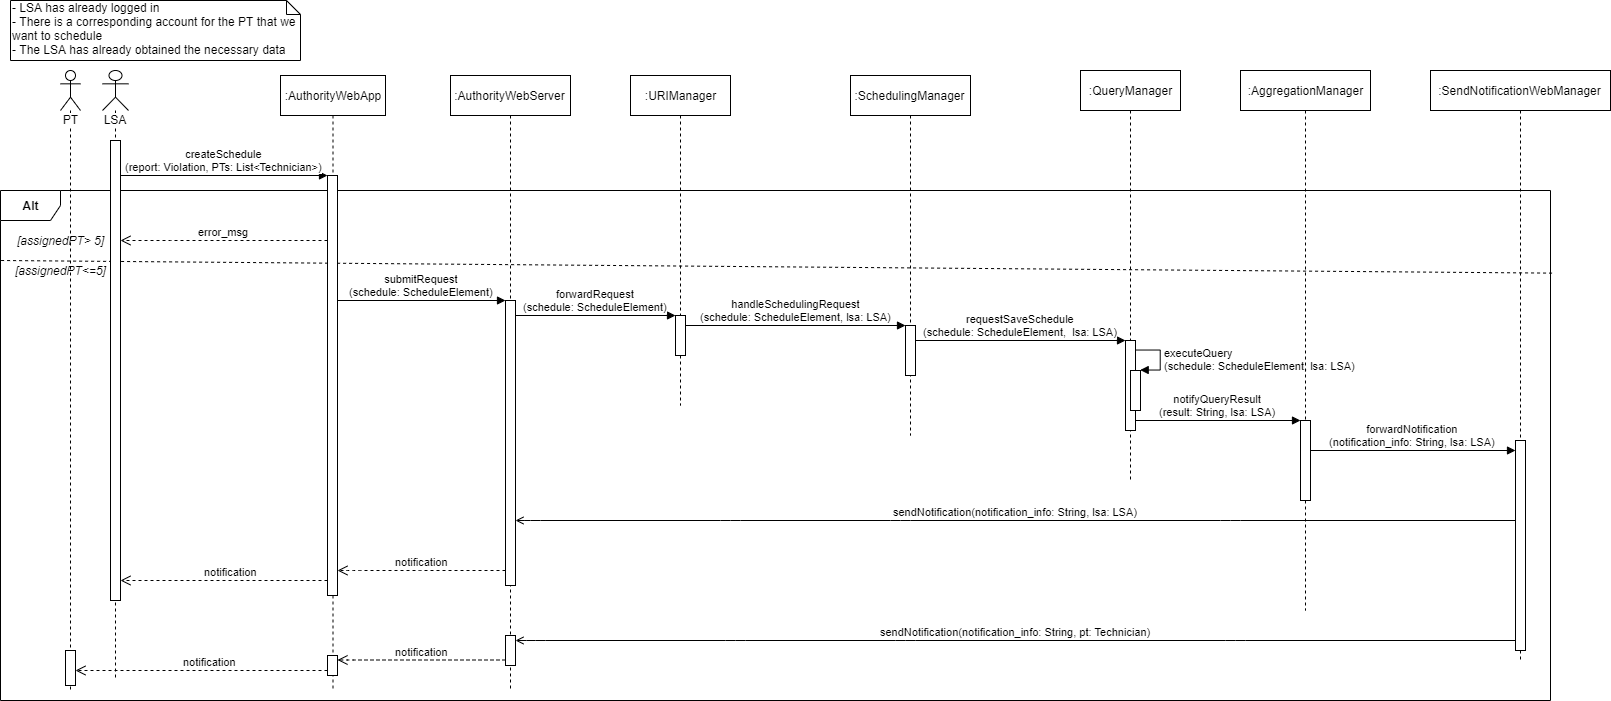
\includegraphics[width=1\textwidth]{Images/UML_diagrams/Sequence_Diagrams/Schedule_PT_sd.png}
  \caption{Schedule Police Technician sequence diagram}
  \label{fig:schedule_PT_sd}
\end{figure}
This sequence diagram represents the process done by the LSA of scheduling Police Technicians to a specific report. For the sake of clarity this sequence diagram has in its prerequisites the fact that the LSA already collected the data about new reports and his PTs. Formally the web app will have to execute a request for the latest reports (i.e. status pending) and the PTs associated with the LSA. This is only a simplification to avoid writing in the sequence diagram all the process to retrieve this data, which is very similar to a mining request. Under this assumption the LSA can then select a report on which compile a schedule of PTs. Before the confirmation of the schedule, the web app checks that no more than 5 PTs are associated with the report. If this constraint is violated an error message is returned, otherwise the schedule is complete and the web app submits a request that, through the AuthorityWebServer and the URIManager, is delivered to the SchedulingManager component. This component validates the schedule and asks to the QueryManager to save this association. The QueryManager saves the schedule, and through the SendNotificationWebManager, notifies the LSA that the assignment has been correctly registered.
